\chapter*{Introducción}\label{chapter:introduction}
\addcontentsline{toc}{chapter}{Introducción}

En la era del \textit{big data}, la capacidad de analizar e interpretar datos complejos de trayectorias humanas se ha convertido en un elemento esencial para comprender y gestionar dinámicas sociales, urbanas y ambientales. Este análisis, impulsado por datos recolectados a través de la telefonía móvil, no solo permite identificar patrones de movilidad humana, sino que también informa la planificación urbana, optimiza el transporte y guía la formulación de políticas públicas. Sin embargo, estos datos suelen ser incompletos o dispersos debido a factores como la pérdida de señal o limitaciones en las capacidades de seguimiento, lo que hace imprescindible desarrollar estrategias eficaces para su completamiento.

En contextos de desarrollo como Cuba, donde la digitalización está en crecimiento, pero los recursos y datos disponibles son limitados, los datos recolectados mediante la telefonía móvil ofrecen una oportunidad invaluable. No obstante, la dispersión, incompletitud e irregularidad en el tiempo de los datos, debido a apagones y averías en el sistema de telecomunicaciones, dificultan en gran medida este proceso. Dentro de este panorama, el completamiento de trayectorias humanas a partir de datos escasos representa un reto significativo en nuestro país, de ahí la necesidad de desarrollar soluciones adaptadas a nuestras particularidades.

Los enfoques tradicionales para el completamiento de trayectorias humanas han estado basados principalmente en técnicas como la interpolación lineal, los modelos basados en patrones históricos, el \textit{clustering} de trayectorias y el uso de factorización de matrices o tensores. Estas técnicas, aunque útiles en ciertos contextos, presentan limitaciones significativas. Por ejemplo, la interpolación lineal, aunque computacionalmente eficiente, no captura patrones complejos de movilidad; los modelos históricos y los métodos de \textit{clustering} tienden a fallar en entornos con alta variabilidad o datos limitados; y la factorización de matrices, si bien efectiva para manejar datos dispersos como los registros de llamadas, no logra modelar adecuadamente las dinámicas temporales complejas.

Por otro lado, el análisis de trayectorias humanas como secuencias espaciotemporales resulta especialmente prometedor para enfoques modernos como los basados en arquitecturas de \textit{transformers} \cite{vaswani2017attention}. Estas arquitecturas destacan por su capacidad para modelar secuencias de manera eficiente, identificando relaciones clave entre los puntos de la trayectoria. Este enfoque permite aprovechar la estructura temporal y espacial de los datos para extraer patrones relevantes, ofreciendo una ventaja significativa frente a métodos tradicionales que no consideran estas interdependencias de forma explícita.

Aunque las arquitecturas basadas en \textit{transformers} han mostrado gran capacidad para analizar secuencias complejas, su aplicación en contextos específicos, como el caso cubano, requiere una exploración cuidadosa de las características particulares de los datos disponibles. En Cuba, la telefonía móvil, a través de la Empresa de Telecomunicaciones de Cuba (Etecsa), ha generado un conjunto de registros espaciotemporales que se emplean en estudios de movilidad desde 2020 por el Centro de Sistemas Complejos en la Facultad de Física de la Universidad de la Habana. Estos datos, aunque menos precisos y abundantes que los proporcionados por empresas internacionales como Google, han demostrado su utilidad en contextos críticos, como la gestión de la pandemia de SARS-CoV2. Esto plantea el desafío de evaluar cómo técnicas avanzadas pueden maximizar el valor informacional de estos datos locales, sentando las bases para abordar problemas específicos de movilidad y toma de decisiones en el país.

A partir de lo discutido anteriormente, podemos identificar como \textbf{problema científico} que los métodos tradicionales no son capaces de completar trayectorias humanas con precisión en escenarios de datos dispersos e irregulares, como ocurre en Cuba. La \textbf{hipótesis} de trabajo es que el uso de un modelo basado en \textit{transformers} permitirá superar estas limitaciones al capturar de manera más efectiva las relaciones espaciotemporales presentes en los datos y proporcionar un completamiento de trayectorias más preciso.

Por tanto, y teniendo en cuenta los datos disponibles en el Centro de Sistemas Complejos y las condiciones establecidas con la empresa de telecomunicaciones para su uso, esta investigación aborda el problema de completar trayectorias de movilidad humana a partir de registros de telefonía móvil en Cuba. A diferencia de trabajos previos, se evalúa la aplicabilidad y desempeño de TrajBERT \cite{si2023trajbert}, un modelo basado en la arquitectura de \textit{transformers} , adaptado a las particularidades locales. Este enfoque busca avanzar en el desarrollo de modelos de movilidad más precisos, explorando tanto sus fortalezas como sus limitaciones en entornos similares.

En este marco, el objetivo general del estudio es investigar la aplicabilidad y adaptabilidad de TrajBERT para el completamiento de trayectorias humanas en el contexto cubano, utilizando datos recolectados mediante telefonía móvil.

 Para lograr este fin, se proponen los siguientes objetivos específicos:

 \begin{enumerate}
    \item Explorar el uso de datos de telefonía móvil para estudios de movilidad humana a nivel global, específicamente en Cuba, e investigar la literatura relacionada con el tema y las herramientas tecnológicas utilizadas, como el aprendizaje profundo y las arquitecturas basadas en \textit{transformer}.
    \item Analizar las fortalezas y debilidades del modelo TrajBERT en el contexto del completamiento de trayectorias, mediante la evaluación de su arquitectura y capacidades técnicas.
    \item Implementar TrajBERT utilizando una base de datos de trayectorias cubanas para evaluar su desempeño en la recuperación de trayectorias individuales.
    \item Comparar los resultados obtenidos por TrajBERT con los de métodos tradicionales y soluciones existentes en el campo, en cuanto a las diferencias de precisión y efectividad.
\end{enumerate}

% \section*{Datos de telefonía móvil}

% El crecimiento sostenido de la población humana, junto con su concentración en áreas urbanas y el aumento de su movilidad, ha planteado retos significativos para la adaptación de los sistemas sociales y demográficos. Estas dinámicas impactan directamente en la planificación y desarrollo de políticas públicas, ya que entender los patrones de movilidad resulta crucial para abordar problemas en diversas áreas. Por ejemplo, en la planificación del transporte, conocer cómo se desplazan las personas permite diseñar redes de carreteras más eficientes y sistemas de transporte público mejor adaptados a las necesidades de la población. En el ámbito de la salud, el modelado de la propagación de enfermedades infecciosas se beneficia de estos datos, ya que facilita la implementación de restricciones y controles más efectivos. Además, en el sector comercial, el geomarketing utiliza los patrones de movilidad para optimizar la distribución geográfica de publicidad y anuncios, maximizando su impacto \cite{asgari2013survey}.

% Históricamente, el análisis de la movilidad humana se basaba en métodos tradicionales como encuestas, observación directa o censos poblacionales. Aunque útiles, estos enfoques presentan limitaciones significativas debido a su elevado costo, frecuencia limitada y dependencia de muestras pequeñas, lo que dificulta obtener una visión integral de los flujos de movilidad \cite{asgari2013survey}. En las últimas décadas, el desarrollo tecnológico ha permitido explorar nuevas fuentes de datos. Algunos estudios como \cite{gong2012gps} hacen uso de los sistemas GPS, que ofrecen una alta precisión en exteriores, sin embargo su uso puede ser intermitente debido al consumo de batería de los dispositivos, y por lo general requieren de la instalación de software específico y la activación del mismo por parte del usuario. Esto implica que los estudios basados en GPS suelan estar limitados a pequeñas muestras. Una alternativa, menos precisa pero mucho más abarcadora, es el uso de datos provenientes de las redes de telecomunicaciones, en particular los registros generados por los teléfonos móviles. Estos dispositivos, que actualmente son utilizados por el 80$\%$ de la población mundial mayor de 10 años y hasta el 90$\%$ en regiones como América y Europa \cite{ITU2024}, recopilan una cantidad masiva de datos vinculados a la actividad de sus usuarios \cite{toole2015path} que se requieren para el correcto funcionamiento de la red.

% Los registros de telefonía móvil incluyen información como la identificación anónima del usuario, la ubicación de las radio bases con las que interactúan sus dispositivos y marcas temporales, permitiendo rastrear trayectorias de movilidad en tiempo real. Esto convierte a los teléfonos móviles en una plataforma de censado masivo de la actividad humana \cite{doyle2014population}, que no solo es económica y escalable, sino también capaz de proporcionar una visión general de los desplazamientos individuales y colectivos. Estas trayectorias ofrecen información valiosa para el análisis de la movilidad humana, contribuyendo a la toma de decisiones en múltiples campos y representando un recurso crucial para la investigación y el desarrollo de soluciones basadas en datos.

% \subsection*{Registros de Telefonía Móvil}

% Una red de telefonía celular se compone de una infraestructura de radio desplegada en áreas denominadas celdas, cada una equipada con al menos una estación base transmisora-receptora fija (BTS, por sus siglas en inglés, \textit{base transceiver station}) \cite{sharma2012cell}. Estas estaciones permiten establecer conexiones inalámbricas entre los terminales de los usuarios y la red en cualquier momento. Las interacciones generadas entre los dispositivos móviles y las BTS se almacenan en registros que contienen información clave, como identificadores de los usuarios y de las estaciones a las que se conectan \cite{yuan2013characterizing}. La estructura y el tipo de registros generados pueden variar según la tecnología utilizada por el proveedor de la red, aunque ciertos estándares han sido adoptados de manera general \cite{durive2021sistema}.

% Entre los registros de mayor interés para estudios de movilidad se encuentran los Call Detail Records (CDR) y los Location Update Records (LUR) \cite{gutierrez2020como}. Los CDR se generan durante eventos específicos, como llamadas, mensajes o conexiones a la red, y son comúnmente utilizados para la facturación de los usuarios, lo que asegura su almacenamiento por largos períodos. Estos registros incluyen información como identificadores de los dispositivos, marcas de tiempo y tipos de eventos, siendo ampliamente utilizados en estudios de movilidad gracias a su disponibilidad. Por otro lado, los LUR son activados por la red en situaciones como cambios de cobertura o períodos de inactividad, proporcionando una mayor resolución temporal al registrar eventos independientes de las actividades de los usuarios. Sin embargo, debido a que no son utilizados para facturación, suelen ser desechados, lo que limita su aplicación en estudios de movilidad \cite{durive2021sistema}.

% A pesar de las diferencias en los eventos que generan estos registros, ambos comparten una estructura de información similar, incluyendo identificadores, eventos, celdas y marcas temporales. Estos datos permiten aproximar las localizaciones de los usuarios en diferentes momentos, aunque la resolución espacial depende de la densidad de las BTS, la cual varía significativamente entre áreas urbanas y rurales \cite{forghani2020cellular}. Al identificar registros con el mismo identificador de usuario, es posible reconstruir trayectorias aproximadas que muestran las posiciones de las estaciones base a las que un dispositivo se conectó mientras se desplazaba \cite{chen2018individual}. En este contexto, una colección de trayectorias derivadas de datos de telefonía móvil puede ofrecer una representación aproximada de la movilidad.

% \subsection*{Desafíos}

% Los datos de redes de telecomunicaciones han revolucionado los estudios de movilidad humana al proporcionar grandes volúmenes de información que superan las limitaciones de métodos tradicionales como las encuestas. Aunque estos datos han abierto nuevas posibilidades para investigar patrones de movilidad, también presentan desafíos significativos.

% Uno de los principales retos es garantizar la privacidad de los usuarios, la cual ha recibido mucha atención en los años recientes. La protección de información sensible ha llevado a restricciones en el acceso a los registros, incluso cuando están anonimizados. Por ejemplo en \cite{tesselkin2017estimation} se presenta un modelo de red de transporte en forma de cadena de Markov para la estimación de las matrices origen-destino (O-D). Con cierta similitud, en \cite{pourmoradnasseri2019od} un modelo de Markov de segundo orden es empleado bajo la premisa de investigar patrones de movilidad humanos a partir de telefonía celular. Resultando de interés, en particular, la determinación de matrices O-D y el completamiento de trayectoria.

% A pesar de los avances, el balance entre el aprovechamiento de los datos y la protección de la privacidad sigue siendo una barrera crítica en la investigación, especialmente en contextos donde el acceso a datos es fundamental para obtener resultados significativos.

% % % \subsection*{Antecedentes}

% % % Este último apartado, el de el completamiento de trayectorias, ha recibido especial atención debido a las limitaciones relacionadas con la resolución temporal y espacial de los registros de telefonía móvil. Se ha presentado un amplio grupo de metodologías orientadas hacia este problema, frecuentemente uniendo datos de telefonía con la estructura de alguna red de transporte. Contando estas metodologías con un grupo de limitaciones.

% % % Se pueden encontrar algunas metodologías de completamiento basadas en interpolación, como el caso de [20]. La interpolación, en general, es precisa cuando la densidad de puntos es elevada, lo cual no suele ser el caso de los registros de telefonía, ademas de que no suele usar información de trayectorias similares para el completamiento. De forma similar [21] realiza el completamiento uniendo nodos para lograr el camino mas corto dentro de una red de transito a la cual son mapeadas las localizaciones de los registros y Vajakas et al. [22] propone un completamiento basado en asignar el camino mas rápido entre los dos puntos de la red de transito de la cual se tengan registros consecutivos.

% % % Por su parte, [23] utiliza la periodicidad en la movilidad humana y la factorización de tensores para completar trayectorias individuales, para lo cual se necesitan datos de un mismo usuario por un largo periodo de tiempo. Otros trabajos orientados al completamiento de trayectorias complementan los registros con información topológica [15] o información sobre el \textit{handoff} entre torres [24].

% % % El marco GRFTrajRec aborda los desafíos de datos de trayectorias urbanas de baja frecuencia mediante una innovadora representación basada en grafos que integra dimensiones de red y trayectoria. Con un modelo seq2seq sensible a intervalos espaciotemporales, GRFTrajRec captura atributos esenciales en los puntos de trayectoria, permitiendo restaurar puntos GPS ausentes con alta precisión.

% % % Una buena parte de los trabajos orientados al completamiento de trayectorias de movilidad utilizan técnicas de \textit{machine learning} o redes neuronales artificiales (ANN, por \textit{artifcial neural network}). Por ejemplo, en [25] se presenta una métodología para reconstruir trayectorias a partir de imágenes, utilizando una ANN para refnar las trayectorias después de una etapa de \textit{clustering}. Zhang et al. [26] propone una red neuronal profunda combinando redes convolucionales, secuenciales y dos mecanismos de atención para estimar localizaciones en exteriores a partir de información de la red de telefonía que incluye datos de la intensidad de la señal del usuario respecto a diferentes torres. La trayectoria se reconstruye a partir de las localizaciones estimadas a partir de una técnica de \textit{map-matching} presentada en [27].

% \subsection*{Historia en Cuba}

% La Empresa de Telecomunicaciones de Cuba, Etecsa, es la única empresa en el territorio nacional que provee servicios de telefonía móvil e Internet. A pesar de grandes avances los últimos años, estos servicios demoraron más tiempo para hacerse populares y accesibles a la mayor parte de la población cubana respecto a la media mundial \cite{durive2021sistema}. Como consecuencia directa, la experiencia con el uso de datos de la red de telefonía celular para estudios de movilidad en Cuba esta limitada a años recientes.

% Según se relata en \cite{durive2021sistema}, en 2018 comienza un esfuerzo por parte de investigadores del actual Centro de Sistemas Complejos de la Facultad de Física de la Universidad de La Habana para acceder a los registros de telefonía celular con el objetivo de extraer analítica que enriqueciera los procesos de toma de decisiones por parte de las autoridades de salud, planificación del transporte y estudios socio-demográficos, etc. Obteniéndose el acceso a registros de tipo LUR a partir del año 2020, acordándose con Etecsa la firma de un acuerdo de confidencialidad con la universidad y el compromiso de respetar una serie de métodos de seguridad entre los que figura que:

% \begin{itemize}
%     \item los datos de LUR son almacenados en servidores de Etecsa, dentro de la red de la compañía;
%     \item los datos son almacenados sin identificadores de usuarios, como nombre, teléfono o IMSI;
%     \item ningún dato de granularidad individual puede sustraerse de la red de la empresa;
%     \item ningún procedimiento de ingeniera inversa o \textit{de-anonymization} puede usarse;
%     \item los datos se entregan con fines de investigación y solo pueden usarse para estos fines;
%     \item Etecsa emite por escrito autorización para la divulgación de los resultados obtenidos.
% \end{itemize}

% Etecsa ha desplegado más de 1,500 radiobases en Cuba, con una distribución heterogénea que refleja la densidad de usuarios, concentrándose en áreas urbanas. Para proteger la ubicación precisa de estas torres, se adoptó una estrategia que agrupa torres cercanas en zonas densas y ajusta ligeramente su posición en zonas rurales, reduciendo el número a 795 pseudo-torres con ubicaciones GPS compartidas. Estas pseudo-torres se emplean en estudios de movilidad mediante zonas de cobertura definidas con celdas de Voronoi, funcionando de manera similar a las torres reales para los análisis realizados.

% El estudio de la movilidad poblacional a partir de los registros LUR de la empresa Etecsa está amparado por la legislación cubana. En particular la Ley de protección de Datos Personales \cite{cuervo2022resolucion}, del 2022, define lo que se consideran datos personales (que incluye los datos generados por sistemas tecnológicos como los teléfonos) y las reglas para su uso. Estipula que dichos datos pueden usarse por razones de bienestar general si se someten previamente a un procedimiento de disociación, como el antes mencionado.

% El valor social de comprender y usar estos datos quedó demostrado ampliamente cuando en medio de la pandemia de SARS-CoV2 a partir de marzo de 2020, el sistema de salud y el gobierno cubanos pudieron disponer de modelos de movilidad para evaluar la efectividad de las medidas de limitación de movimiento que se implementaron. Es importante resaltar que, durante ese mismo período, la mayor parte de los gobiernos del mundo usaron métricas semejantes para entender la epidemia y sus consecuencias. En muchos casos, los modelos de movilidad provinieron de empresas como Google, que amparada por la urgencia médica mundial, puso a disposición de los investigadores modelos de movilidad basados en la detección de posicionamiento de los usuarios a partir de los metadatos generados por sus aplicaciones. Es de señalar que Google excluyó a Cuba de la lista de países que podían acceder a dichos datos, como se muestra en la figura \ref{fig:google_exclusion}.

% \begin{figure}[!htb] \centering 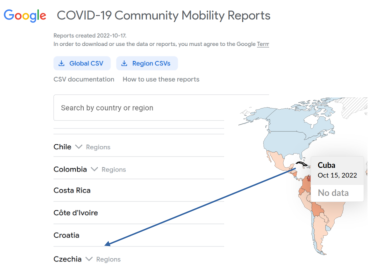
\includegraphics[width=0.5\textwidth]{Graphics/google_exclusion.pdf} \caption{Cuba excluida por Google en el acceso a datos de movilidad} \label{fig:google_exclusion} \end{figure}

% Si bien los modelos de movilidad generados por el Centro de Sistemas Complejos, de acuerdo con Etecsa, fueron de gran utilidad, es importante señalar que dichos datos tienen menos precisión y menos abundantes que los que disponen empresas como Google, Facebook y otras.

% Una de las enseñanzas de la pandemia y de la posterior aplicación de estos datos al estudio de la movilidad poblacional es que no se puede esperar a tener situaciones críticas para decidirse a usar estos métodos de Big Data. Esencialmente, aunque el posible uso y valor de estos datos sea bastante obvio, en los detalles de cómo extraer valor informacional radica un gran reto. Es importante crear una base científica y tecnológica que permita, ante necesidades concretas, saber las potencialidades de estos datos, si permiten o no enfrentar la tarea en cuestión, y la precisión de los mismos.

% % % En los últimos años, diversas investigaciones han explorado métodos para el completamiento y la predicción de trayectorias, abarcando desde técnicas clásicas de interpolación hasta enfoques más recientes de aprendizaje profundo. La competencia HuMob (Human Mobility) Challenge ha tenido un gran impacto en este campo, ya que se propone anualmente romper el estado del arte de los modelos computacionales para la predicción de patrones de movilidad humana. Lamentablemente, la mayoría de los estudios están casi siempre orientados a entornos con abundancia de datos, dejando una brecha en la literatura sobre contextos con datos limitados. Destacan entonces enfoques como el de GRFTrajRec con una representación de trayectorias basada en grafos, la cual mejora la comprensión de las interacciones entre trayectorias y redes viales. Este sistema, usando un modelo seq2seq basado en intervalos espaciotemporales, ha demostrado aumentar la precisión y la consistencia espacial en las predicciones utilizando datos reales. Otra investigación basada en factorización tensorial, en conjunto con datos de registros de llamadas o CDR (por sus siglas en ingles, \textit{call detail records}), permite reconstruir trayectorias individuales con alta precisión, incluso con solo el 1$\%$ de los datos originales.

% % % El uso de datos de telefonía en Cuba ha permitido analizar patrones de movilidad en diversas situaciones, como durante la pandemia de COVID-19, y ha sido fundamental en la integración de modelos para la propagación de epidemias. De igual forma, estudios han aprovechado estos datos para actualizar áreas de ubicación y comprender los flujos de movilidad entre zonas de transporte, lo que contribuye significativamente a la toma de decisiones y al control de crisis.

% \section*{Objetivos y estructura del documento}

% Teniendo en cuenta los datos disponibles en el Centro de Sistemas Complejos y las condiciones pactadas con la empresa de telecomunicaciones para el uso de los mismos, esta investigación se plantea atender el problema de completar trayectorias de movilidad humana a partir de registros de telefonía móvil, utilizando métodos que consideren la baja densidad de los datos. El objetivo fundamental es el de contribuir a la creación de modelos de movilidad más preciso a partir del completamiento de datos que suelen ser imprecisos e incompletos.

% A diferencia de investigaciones cubanas anteriores, este trabajo se centra en evaluar la aplicabilidad y el desempeño de TrajBERT \cite{si2023trajbert}, un modelo basado en la arquitectura de \textit{transformer} \cite{vaswani2017attention} que permite aprovechar la información espaciotemporal. Este estudio se enfoca en adaptar el modelo a las particularidades locales, al emplear datos cubanos recolectados mediante telefonía móvil. Finalmente, se busca identificar tanto las fortalezas como las limitaciones del modelo, contribuyendo al avance del conocimiento en el campo.

% Por tanto el objetivo general que rige este estudio es investigar la aplicabilidad y adaptabilidad del modelo TrajBERT para el completamiento de trayectorias humanas en el contexto cubano, utilizando datos recolectados mediante telefonía móvil.

% Para cumplir el objetivo general se definen los siguientes objetivos específicos:

% \begin{enumerate}
%     \item Explorar el uso de datos de telefonía móvil para estudios de movilidad humana a nivel global, específicamente en Cuba, e investigar la literatura relacionada con el tema y las herramientas tecnológicas utilizadas, como el aprendizaje profundo y las arquitecturas basadas en \textit{transformer}.
%     \item Analizar las fortalezas y debilidades del modelo TrajBERT en el contexto del completamiento de trayectorias, mediante la evaluación de su arquitectura y capacidades técnicas.
%     \item Implementar TrajBERT utilizando una base de datos de trayectorias cubanas para evaluar su desempeño en la recuperación de trayectorias individuales.
%     \item Comparar los resultados obtenidos por TrajBERT con los de métodos tradicionales y soluciones existentes en el campo, en cuanto a las diferencias de precisión y efectividad.
% \end{enumerate}

La estructura de la tesis está diseñada para cumplir con los objetivos planteados mediante tres capítulos interrelacionados.

El Capítulo 1 se centra en la revisión de la literatura y las herramientas tecnológicas utilizadas, abordando el objetivo de investigar las bases teóricas y metodológicas del tema. Aquí se analizan los avances recientes en completamiento de trayectorias, destacando tanto métodos tradicionales como modernos, además de explorar en profundidad las arquitecturas basadas en \textit{transformer} y sus aplicaciones en el aprendizaje profundo. Esto establece un marco teórico sólido que respalda el desarrollo posterior de la tesis.

El Capítulo 2 aborda el análisis y la implementación del modelo TrajBERT, cumpliendo con los objetivos relacionados con la evaluación de sus fortalezas y debilidades, así como su implementación práctica. Posteriormente, se implementa el modelo utilizando la base de datos pública de la competencia HuMob (Human Mobility) Challenge 2023, lo que incluye el preprocesamiento de datos, entrenamiento del modelo y evaluación de su desempeño en la recuperación de trayectorias individuales mediante métricas específicas.

Finalmente, el Capítulo 3 se enfoca en la implementación y evaluación del modelo TrajBERT utilizando datos de trayectorias cubanas, permitiendo cumplir con el objetivo de contextualizar su desempeño en un entorno local y comparar sus resultados con métodos tradicionales y soluciones existentes en el campo. Este capítulo concluye con un análisis sobre las ventajas y limitaciones del modelo TrajBERT cuando se aplica a datos locales, ofreciendo recomendaciones para futuras investigaciones en el área.

Esta estructura garantiza que cada objetivo se aborde de manera sistemática y que los capítulos estén interconectados de forma coherente para proporcionar resultados concluyentes.